\appendix
\section*{Appendix}
\label{sec:appendix}

\section{Detailed Role Subtask Telemetry on Stage 3}
\label{sec:app_subtasks}

Figure~\ref{fig:subtasks} and Table~\ref{tab:subtasks_stage3} present comprehensive diagnostic evaluations of role-specific subtask success rates, terminal hacking frequencies, security alert accumulation, and extraction survival on Stage 3 ($35 \times 35$, 3 guards, 2 cameras, 3 locked doors) across all evaluated methods.

\begin{figure}[h]
\centering
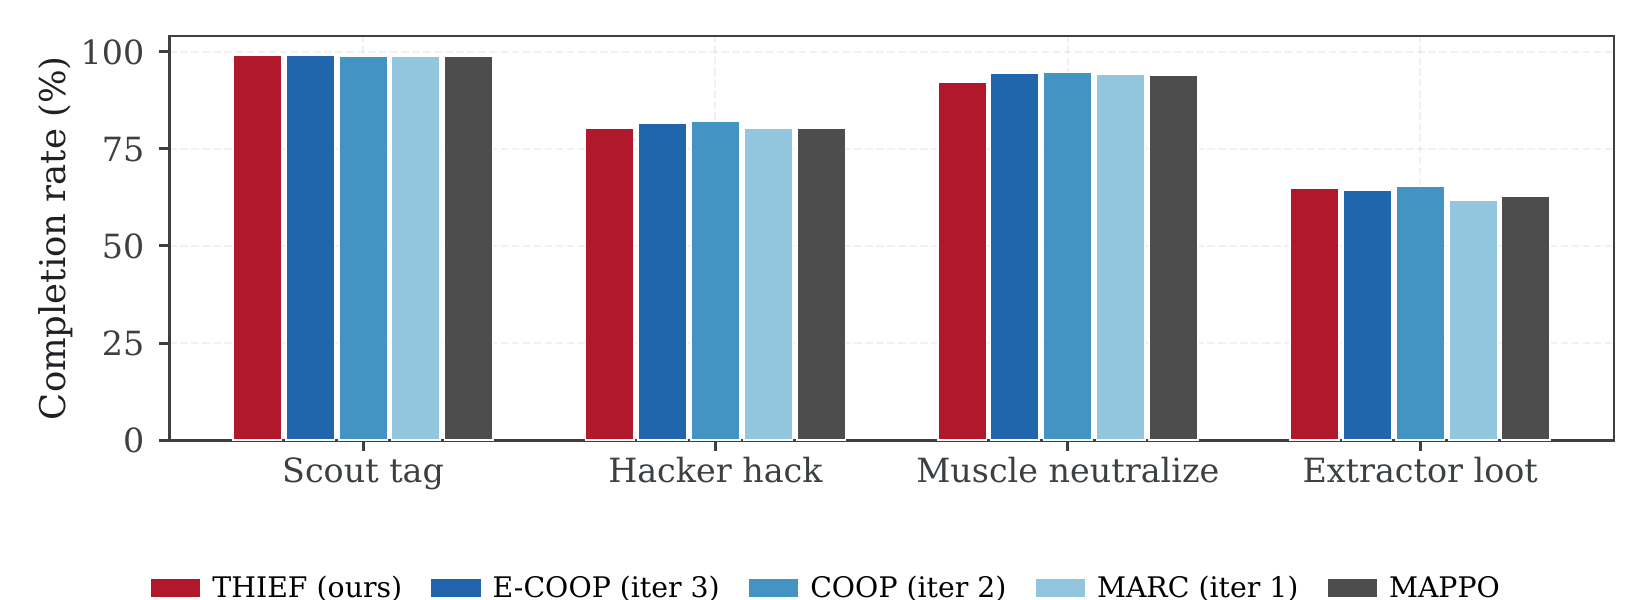
\includegraphics[width=\linewidth]{figures/stage3_subtasks.pdf}
\caption{\textbf{Role Subtask Success Rates on Stage 3.} Grouped bar breakdown of role-specific subtask completion for the method lineage (MARC, COOP, E-COOP, THIEF) against the leading external baseline (MAPPO), evaluated over $N=1,\!000$ episodes across 10 random training seeds ($10,\!000$ episodes per algorithm).}
\label{fig:subtasks}
\end{figure}

% Auto-generated by paper/scripts/generate_tables.py. Do not edit manually.
\begin{table}[htbp]
\centering
\caption{Role subtask completion rates and tactical telemetry on Stage 3 ($35\times 35$, 3 guards, 2 cameras, 3 locked doors). Evaluation over $N=1,\!000$ episodes across 10 random seeds ($10,\!000$ episodes total per algorithm). Partitioned into our iterative development lineage versus external baselines. Bold denotes highest completion rate or lowest alarm overall.}
\label{tab:subtasks_stage3}
\vspace{0.04in}
\footnotesize
\setlength{\tabcolsep}{2.5pt}
\renewcommand{\arraystretch}{1.06}
\begin{tabular}{l ccccc cc}
\toprule
\textbf{Method} & \textbf{Scout} & \textbf{Hacker} & \textbf{Muscle} & \textbf{Extractor} & \textbf{Agents} & \textbf{Mean} & \textbf{Mean} \\
 & \textbf{Tag (\%)} & \textbf{Hack (\%)} & \textbf{Neut. (\%)} & \textbf{Loot (\%)} & \textbf{Extracted} & \textbf{Alarm} & \textbf{Steps} \\
\midrule
\multicolumn{8}{l}{\textit{\textbf{Proposed Method Lineage (Ours)}}} \\
\midrule
\textbf{THIEF (Ours, Final)} & \textbf{99.1\%} & 80.3\% & 92.2\% & 65.0\% & 2.37 & 89.1 & 775.3 \\
E-COOP (Iteration 3) & 99.0\% & 81.5\% & 94.5\% & 63.9\% & 2.46 & 86.8 & 859.3 \\
COOP (Iteration 2) & 98.8\% & 81.9\% & \textbf{94.7\%} & \textbf{65.3\%} & \textbf{2.49} & 87.5 & 851.4 \\
MARC (Iteration 1) & 98.8\% & 80.4\% & 94.1\% & 61.8\% & 2.37 & 89.3 & 895.4 \\
\midrule
\multicolumn{8}{l}{\textit{\textbf{External MARL Baselines}}} \\
\midrule
ROMA \cite{wang2020roma} & 99.0\% & \textbf{82.6\%} & 94.5\% & 65.2\% & 2.47 & 89.0 & 863.6 \\
RODE \cite{wang2021rode} & 98.7\% & 78.3\% & 94.0\% & 59.5\% & 2.24 & 98.8 & 913.0 \\
MAPPO \cite{yu2022surprising} & 98.8\% & 80.5\% & 94.0\% & 62.6\% & 2.39 & 89.4 & 889.1 \\
H-MAPPO \cite{vezhnevets2017feudal} & 96.6\% & 40.5\% & 92.8\% & 21.4\% & 0.86 & \textbf{86.6} & 1307.1 \\
COMA \cite{foerster2018counterfactual} & 98.7\% & 74.0\% & 93.5\% & 55.6\% & 2.03 & 92.8 & 985.5 \\
\bottomrule
\end{tabular}
\end{table}


\section{Component Micro-Ablations of THIEF}
\label{sec:app_ablation}
To isolate the contribution of each core mechanism, we evaluate THIEF standalone (fresh initialization, identical per-stage budgets and hyperparameters) on two diagnostic stages: Stage 2 ($25 \times 25$), where expert spawning is actively triggered across training, and Stage 4 ($50 \times 50$), the long-horizon regime in which final claims are evaluated. Results are evaluated over $1,\!000$ held-out episodes per seed across random training seeds (Table~\ref{tab:ablations}).

The ablated variants are:
\begin{itemize}[leftmargin=*,nosep]
    \item \textbf{w/o warmup} ($\tau_{\text{iso}}=0$): newly spawned specialists skip isolated sandbox environments and join the global bidding pool immediately with uncalibrated critics.
    \item \textbf{w/o Fisher geometry}: parent recombination uses uniform parameter averaging with isotropic noise, removing curvature weighting and inverse-Fisher exploration scaling.
    \item \textbf{clone-best-parent}: the specialist actor is a perturbed copy of the best parent (no pool recombination, no deficit gradient push), isolating recombination from single-parent cloning.
    \item \textbf{w/o load balancing} ($\alpha_{\text{bal}}=0$): the load-balancing regularizer of Section~\ref{sec:thief} is removed.
    \item \textbf{w/o hysteresis} ($\epsilon=0$): the routing barrier is disabled, allowing unconstrained per-step switching.
    \item \textbf{fixed-schedule spawning}: the win-rate plateau trigger is bypassed in favor of spawning on a fixed update cadence.
\end{itemize}
All variants are trained and evaluated with identical per-stage budgets and hold-out protocols. The first four rows (full THIEF, w/o warmup, w/o Fisher geometry, clone-best-parent) aggregate 10 random seeds per stage; the w/o load balancing, w/o hysteresis, and fixed-schedule variants use a 3-seed diagnostic budget (seeds 0--2), so their standard errors are correspondingly larger and no cross-variant significance is claimed for them.

\InputIfFileExists{tables/ablation}{}{}

\section{Environment Implementation \& Engineering Details}
\label{sec:app_env}
The HEIST simulation engine is developed in native Rust to eliminate Python GIL bottlenecks during multi-agent pathfinding and raytraced field-of-view perception:
\begin{itemize}[leftmargin=*,nosep]
    \item \textbf{Raytraced Line of Sight:} For each agent coordinate, ray traversal is computed along 8 cardinal and diagonal directions. Rays terminate upon encountering perimeter or interior room walls, populating visible tiles into egocentric observation arrays with value $-1$ for occluded fog-of-war tiles.
    \item \textbf{Adversarial Guard Pathfinding:} Guard pathfinding uses a breadth-first search (BFS) queue executed over cached grid obstacle bitmasks. Guard investigation states pathfind toward the last-known coordinate of spotted agents.
    \item \textbf{Zero-Copy PyTorch Sharding:} Simulation steps execute across parallel environments using Rayon worker threads. Observations, rewards, done flags, and action masks are copied directly into pre-allocated contiguous CUDA/CPU tensors.
\end{itemize}

\section{Full Hyperparameter Specifications}
\label{sec:app_hyperparameters}
Table~\ref{tab:hyperparameters} provides the universal hyperparameters shared across all algorithms. The centralized critic input dimensionality of $2,\!550 + 4 + 2$ decomposes as: $6$ global scalars (step counter, alarm, terminal/loot/extraction flags, extraction countdown) $+\; 50 \times 50 = 2,\!500$ grid cells $+\; 8$ agent coordinates $+\; 12 \times 2 = 24$ guard coordinates (unused guard slots padded with $-1$) $+\; 12$ guard-neutralization flags $= 2,\!550$, plus the $4$-dimensional role embedding and $2$-dimensional mission compass. Because the $50 \times 50$ grid canvas and the 12 guard slots are fixed capacity across all curriculum stages (cells outside the active stage's floorplan hold the wall token), this input dimensionality is identical at every stage, which is precisely what allows critic checkpoints to transfer between curriculum stages without architectural modification.

% Universal training and architectural hyperparameters.
\begin{table}[t]
\centering
\caption{Universal training and architectural hyperparameters across all evaluated MARL algorithms (verified against the reference implementation). Environment- and algorithm-specific values are noted where they differ.}
\label{tab:hyperparameters}
\vspace{0.06in}
\small
\setlength{\tabcolsep}{4.0pt}
\renewcommand{\arraystretch}{1.08}
\begin{tabular}{ll}
\toprule
\textbf{Hyperparameter} & \textbf{Value} \\
\midrule
Actor Network Architecture & 2-layer MLP ($[49+4+2] \rightarrow 64 \rightarrow 64 \rightarrow 6$), Tanh \\
Critic Network Architecture & 2-layer MLP ($[2,\!550+4+2] \rightarrow 64 \rightarrow 64 \rightarrow 1$), Tanh \\
Optimizer & Adam ($\text{lr} = 2.5 \times 10^{-4}$, $\epsilon = 10^{-5}$) \\
PPO Clip Ratio ($\epsilon_{\text{clip}}$) & 0.20 \\
Discount Factor ($\gamma$) & 0.99 \\
GAE Parameter ($\lambda_{\text{gae}}$) & 0.95 \\
PPO Epochs per Update & 4 \\
Mini-batches per Update & 4 (batch size / 4) \\
Entropy / Value Coefficients & 0.01 / 0.5 \\
Rollout Horizon ($T$) & 125 steps (all stages) \\
Vectorized Environments & 16 (THIEF, E-COOP); 8 (all other methods) \\
Updates per Stage & 100/100/250/450/800 (16 envs); $2\times$ for 8-env baselines \\
Training Budget per Stage & $2/2/5/9/16 \times 10^5$ env.\ steps (Stages 0--4) \\
\midrule
\multicolumn{2}{l}{\emph{THIEF-specific}} \\
Hysteresis Barrier ($\epsilon$) & 0.05 \\
Plateau Trigger ($\Delta_{\text{win}}$) & $< 0.03$ over last 100 episodes ($\ge 200$ recorded) \\
Spawning Ceiling & suppressed when recent win rate $\ge 0.90$ \\
Incubation Duration ($\tau_{\text{iso}}$) & 10 updates (4 of 16 environments, 25\%) \\
Fisher Decay ($\beta$) & 0.99 \\
Mutation Noise Scale & 0.03 \\
Targeted Deficit Learning Rate ($\eta_{\text{def}}$) & 0.08 \\
Load-Balancing Coefficient ($\alpha_{\text{bal}}$) & 0.01 \\
Dormancy Cull Window ($\tau_{\text{cull}}$) & $\max(60,\, 0.4\,T_{\text{upd}})$ zero-usage updates \\
\bottomrule
\end{tabular}
\end{table}

\paragraph{Hyperparameter Grouping and Sensibility.}
THIEF introduces interdependent hyperparameters beyond the shared PPO backbone; they fall into four mechanism families (all values in Table~\ref{tab:hyperparameters} are held fixed across every seed, stage, and algorithm comparison in this paper): (i) \emph{plateau triggering} --- window $W=100$, threshold $\Delta_{\text{win}}<0.03$, mastery ceiling $0.90$; (ii) \emph{incubation} --- $\tau_{\text{iso}}=10$ updates over a dedicated $25\%$ environment fraction; (iii) \emph{Fisher geometry} --- EMA decay $\beta=0.99$, damping $\lambda=10^{-4}$, deficit step size $\eta_{\text{def}}=0.08$, noise scale $\sigma=0.03$; and (iv) \emph{routing} --- barrier $\epsilon=0.05$, gating temperature $\tau_{\text{gate}}$, balance coefficient $\alpha_{\text{bal}}=0.01$, dormancy threshold $\tau_{\text{cull}}$. Families (ii)--(iv) are exercised in isolation by the micro-ablations of Table~\ref{tab:ablations} (w/o warmup, w/o Fisher geometry, clone-best-parent, w/o load balancing, w/o hysteresis), which probe the qualitative sensitivity of end-to-end performance to removing each mechanism outright; the full THIEF variant degrades gracefully across all of them. We did not run exhaustive per-threshold sweeps (e.g., $\epsilon \in [0.01, 0.10]$ or $\Delta_{\text{win}} \in [0.03, 0.05]$) and flag complete sensitivity analysis as future work.

\section{Compute Environment \& Hardware Throughput}
\label{sec:app_compute}
All benchmark training and evaluation runs were conducted on a single Linux workstation equipped with an NVIDIA GeForce RTX 3080 Ti GPU (12 GB VRAM) and an AMD Ryzen 9 5900X 12-core processor (24 threads). The raw Rust simulation engine sustains approximately $11,\!500$--$12,\!500$ environment steps per second across the curriculum stages (measured over $N=1,\!000$-episode evaluation batches for single-network policies such as MAPPO, MARC, and COMA); end-to-end throughput for multi-expert methods is lower due to per-expert forward passes (e.g., approximately $2,\!400$--$3,\!200$ steps/s for THIEF). Each curriculum stage trains for a fixed budget of $2/2/5/9/16 \times 10^{5}$ environment steps (Stages 0--4, $3.4 \times 10^6$ per seed in total), corresponding to 100/100/250/450/800 PPO updates across all evaluated models using 16 parallel environments uniformly ($16 \times 125 = 2,\!000$ steps per rollout).
